\documentclass{article}

\usepackage{graphicx}
\usepackage{longtable}
\usepackage{subcaption}
\usepackage{caption}
\usepackage{float}
\usepackage{comment}
\usepackage[bookmarks, colorlinks, breaklinks]{hyperref} 
\hypersetup{linkcolor=black, citecolor=black, filecolor=black, urlcolor=black} 
\graphicspath{{./Images/}}

\begin{document}

\begin{figure}
\centering
	
\includegraphics[height=8cm]{Images/polimi_logo}
\end{figure}
	
\title {{\Huge \it SafeStreets} \\ \Large Software Engineering 2 Project - Prof. Matteo Rossi \\ {\bf Design Document}}
\author{Salvatore Fadda - 944786\\Adriano Mundo - 944684 \\ Francesco Rota - 948714
		\\ \\ A.Y. 2019/2020 \\ Version 1.0}
\date{December 9, 2019}	

\maketitle
\newpage

% Index	
\tableofcontents
\newpage

% Introduction - Section 1
\section{Introduction}
	\subsection{Purpose}
	This document represent the {\it Design Document} (DD). It aims at providing an in-depth description of the architecture below {\it SafeStreets} application and its services. It will present a section related to the architectural design with different perspective on the components of the {\it System}, how they interact and how they will be implemented. All the requirements of the RASD document are mapped with the components to explain how they will be satisfied. Finally, a section for the testing plan for Q\&A team is provided.
		
	\subsection{Scope}
	{\it SafeStreets} is a crowd-sourced application that aims at keeping safe the city's streets. The idea behind this service is to allow {\it Users} to notify the {\it Municipality} when a violation occur on the streets under its jurisdiction. The {\it User} can notice and notify the violation by sending a photo of the violation and select the type of violation and; date, time and position are automatically retrieved from the mobile device. {\it SafesStreets} stores all the data and uses an image recognition algorithm to distinguish the content of the image, such as the plate number and other details. \\ \\
	The {\bf Basic Service} allows {\it Users} and {\it Authorities} to mine the information \mbox{collected} by the service, so they can access statistics built from the data. \\ \\
	As {\bf AF1}, the application {\it SafeStreets} identifies potentially unsafe areas and \mbox{suggests} possible interventions to {\it Authorities} to solve the founded issues. \\ \\ 
	As {\bf AF2}. the application {\it SafeStreets} allows the {\it Municipality} to generate \mbox{traffic} tickets directly from the application data. Also, using the data of issued tickets the {\it System} can build statistics and find insights to suggest to {\it Municipality} in order to improve their service.
		
	\subsection{Definitions, Acronyms, Abbreviations}
		\subsubsection{Definitions}
			\begin{itemize}
				\item {\bf Client:} a piece of computer hardware or software that accesses a service made available by a Server. 
				\item {\bf Server:} a computer program or a device that provides functionality and handle the requests of other programs or devices, called Clients. 
				\item {\bf N-Tier:} or multilayer is an architecture in which presentation, application processing, and data management functions are physically separated in n-layers. 
			\end{itemize}
	
	
		\subsubsection{Acronyms}
			\begin{itemize}
				\item {\bf GPS:} Global Positioning System
				\item {\bf API:} Application Programming Interface
				\item {\bf RASD:} Requirements Analysis and Specification Document
				\item {\bf DBMS:} Data Bases Management System
				\item {\bf MVC:} Model-View-Controller
				\item {\bf Q\&A:} Quality and Assurance
				\item {\bf UI:} User Interface
				\item {\bf HTTPS:} Hyper Text Transfer Protocol Secure
			\end{itemize}
		
		\subsubsection{Abbreviations}
			\begin{itemize}
				\item {\bf [Rn]:} n-th Functional Requirement
				\item {\bf A1:} Advanced Function One
				\item {\bf A2:} Advanced Function Two 
			\end{itemize}
	
	
		\subsection{Revision history}
			\begin{table}[ht]
				\centering
				\begin{tabular}{ccc} 
				Version & Date & Description  \\ 
				\hline
		 		\\1.0 & 09/12/2019 & First Delivery
		 		\\
			\end{tabular}
			\caption{Revision History}
			\label{default}
		\end{table}
	
	
		\subsection{Reference Documents}
			\begin{itemize}
				\item Mandatory Project Assignment
				\item RASD Document of {\it SafeStreets} application
			\end{itemize} 
		
		\pagebreak
	
		\subsection{Document Structure}
		The other sections of the Design Document (DD) are organised in this way:
			\begin{itemize}
				\item {\bf Architectural Design} (Section 2): presents an in-depth description of the {\it System}'s architecture. It defines the main components, the relationship between them and the deployment of components. There are different views and levels of analysis of the components plus some subsection useful for identifying how the components interact and for the architectural styles and patterns. 
				\item {\bf User Interface Design} (Section 3): it's a complementary section of what was included in the RASD. It includes the definition of the UX processes through a model that represents the flows between interfaces. 
				\item {\bf Requirements Traceability} (Section 4): a complementary section of what was included in the RASD. It contains all the requirements and shows the relationship between them and design choices done in order to satisfy them. 
				\item {\bf Implementation, Integration and Test Plan} (Section 5): it shows the order of the implementation and integration of all the components and subcomponents, explaining how the application will be tested.
				\item {\bf Effort Spent} (Section 6): it's a section that contains a table for identifying the hours and the effort spent by each team member to deliver the Design Document.
			\end{itemize}
		
		\pagebreak
	
	
% Architectural Design - Section 2
\section{Architectural Design}

	\subsection{Overview}
		\begin{figure}[H]
			\centering
			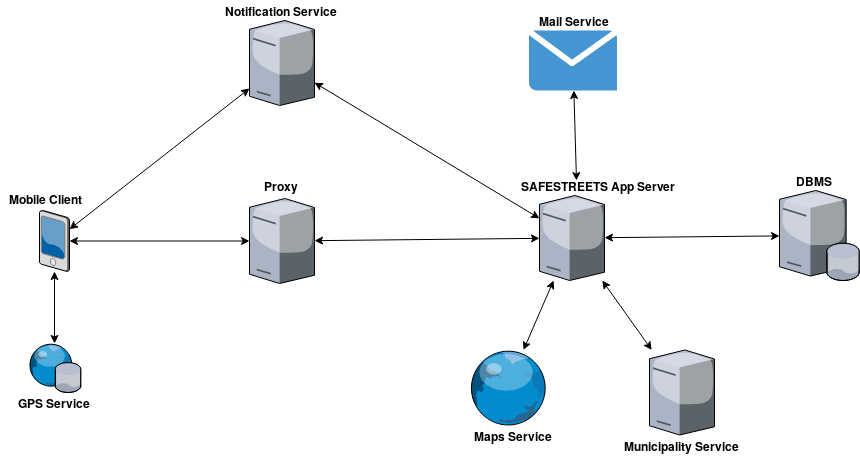
\includegraphics[scale=0.35]{Images/Diagrams/overview_diagram.png}
			\caption{Overview of the System}
		\end{figure}
	The image above shows an high-level overview of the {\it System}'s architecture.
	The components interact with some external services. \\
	The Mobile Client application accesses the GPS service in order to retrieve geographical information and communicates with the Application Server through a Proxy. \\ The Application Server uses an external Notification Service to send notifications directly to the Client. It also uses external services like a Mail service and a Map service to execute all the other functions. Finally, it accesses the Municipality Service to retrieve data and communicate with the Municipality, thanks to the API service offered by the Municipality itself.\\ 
	Further details on the {\it System} components will be explained in the next sections. 		
	\pagebreak	
	
	\subsection{Component View}
		\begin{figure}[H]
			\centering
			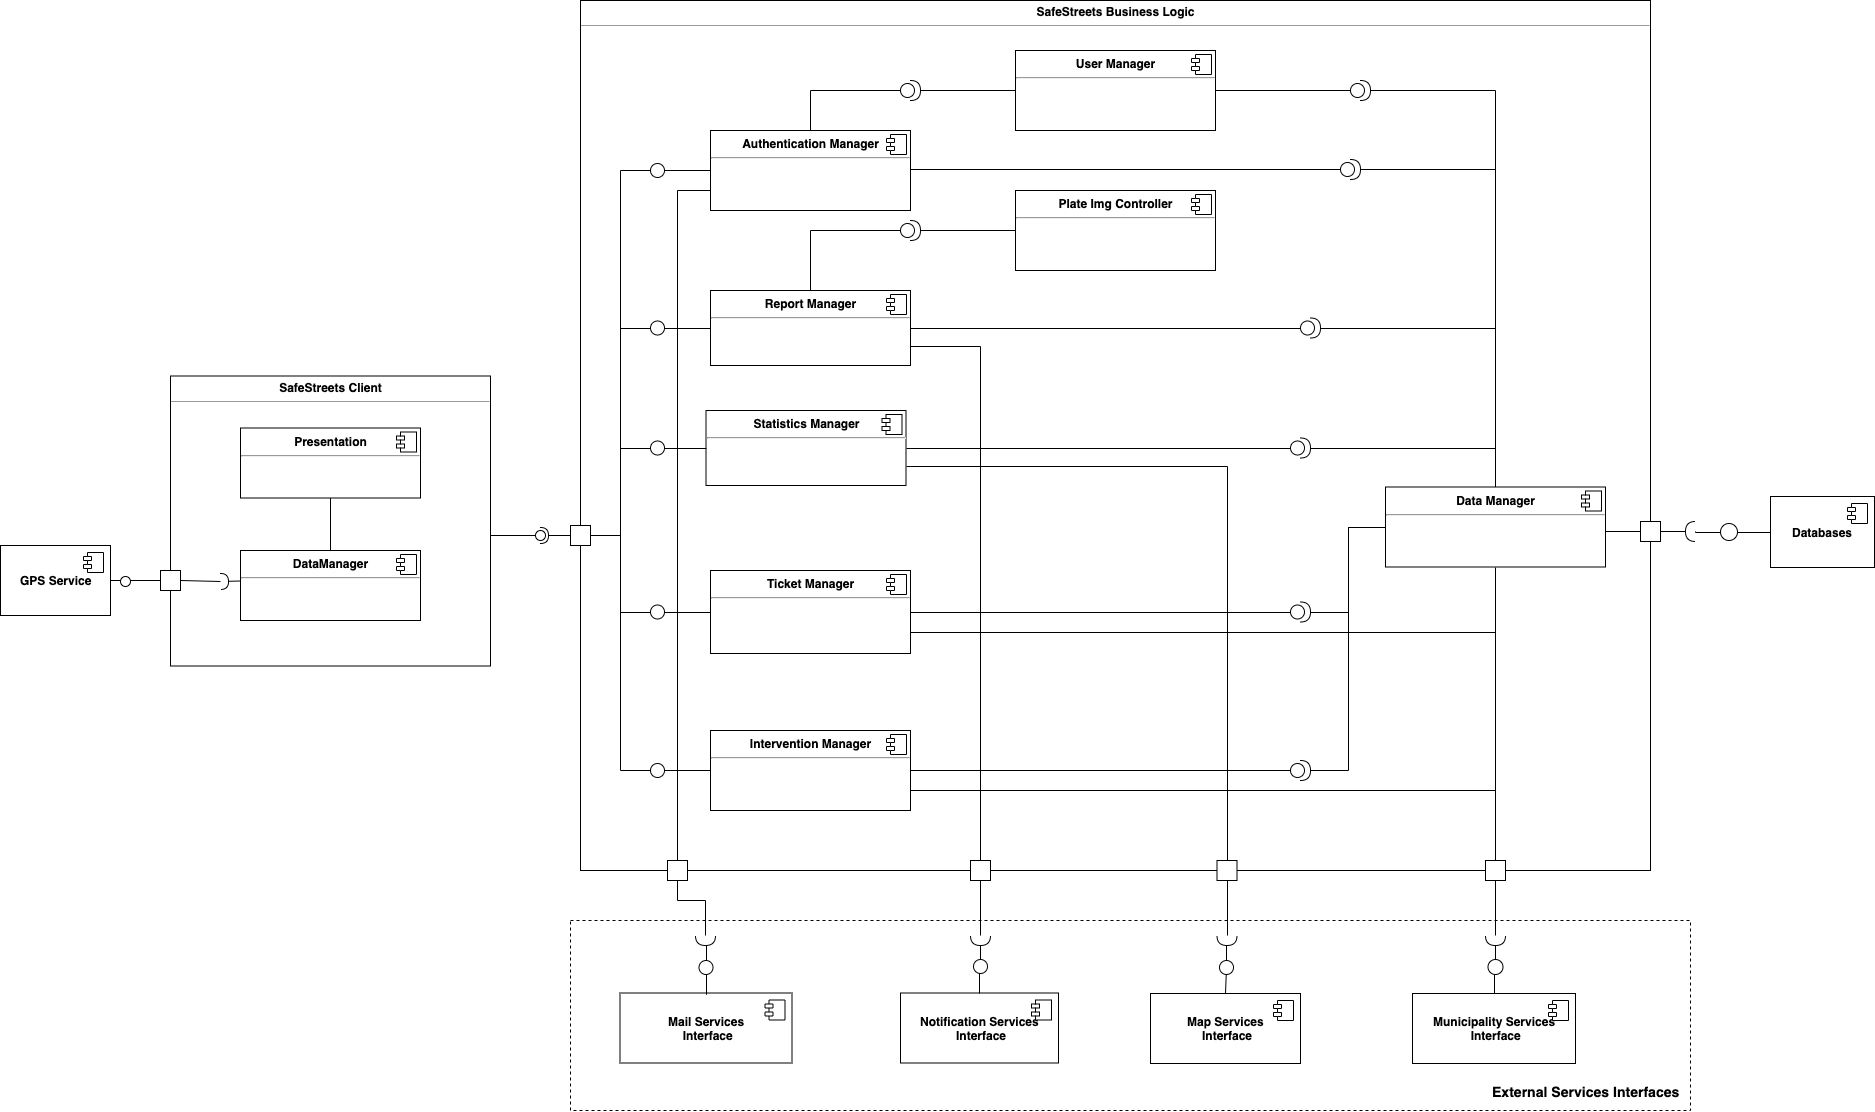
\includegraphics[scale=0.20]{Images/Diagrams/component_diagram.png}
			\caption{{\it SafeStreets} Component Diagram}
		\end{figure}
		The purpose of the UML component diagram is to capture the internal architecture of the {\it System}, showing the structure of components and how they are connected together as a part of larger components. \\
		It's divided in three main components: the {\it SafeStreets} Client Application, the Business Logic and the external Database. \\ 
		Each main component is divided in modular components to provide specific functionalities. Components communicate between each other by providing interfaces with the required information. \\
		This diagram uses assembly connectors for internal interfaces and delegation connectors for external interfaces. 
		\\ \\
		{\bf SafeStreets Client} \\
		This component located on the {\it User}'s device represents the client machines that access to the Business Logic container. Its sub-modules are the Presentation and Data Manager. It is implemented as a thin-client, so does not contain any logic of the {\it System}.
		\begin{itemize}
		\item {\bf Presentation:} this module corresponds to the View of the MVC Pattern, it requires data from the Business Logic to display the correct UI to the {\it User}.
		\item {\bf Data Manager:} this module has to communicate with the GPS Service in order to retrieve the data required from the application. 
		\end{itemize} 
		{\bf SafeStreets Business Logic} \\
		This component contains all the {\it SafeStreets} application logic. It's a module between the Client Application and the Database. It collects together all the components needed to satisfy the application functionalities. In the section below each component will be described.
		\begin{itemize}
		\item {\bf Authentication Manager:} this component contains all the methods needed to access the application, so it's necessary for the purpose of the system authentication. It's responsible for both the registration and log-in process. It continuously interacts with the Database through the Data Manager interface. It guarantees that all the constraints are respected and finally, when you need to confirm to the {\it Users} they have successfully registered, it communicates with the Mail Service Interface to send the confirmation e-mail. 
		\item {\bf User Manager:} this component handles all the functionalities related to the User account, both for simple {\it Users} and {\it Authorities}. Its services are performed by interacting with the Database through the Data Manager. 
		\item {\bf Report Manager:} this component contains the logic needed to perform and handle the violation reported by the {\it User}. Its service are linked to the image loading, the violation indication type and so on. It interacts with another component that's responsible for analysing the image, the Plate Img Controller and stores all the data in the Database through the Data Manager.  Finally, the Report Manager communicates with the Notification Service Interface because it gives a direct feedback to the {\it User} about the loaded image through a push notification.
		\item {\bf Plate Img Controller:} this component handles the request coming from the {\it User} that loads the violation image. The request comes from the Report Manager, in fact the component exposes the methods to verify that the image was not modified by third parties, so it makes a consistency check. In order to do this task, the component runs an image recognition algorithm.
		\item {\bf Statistics Manager:} this component manage and calculate all the statistics that the application is intended to provide to both {\it Users} and {\it Authorities}. It has two main task: retrieve and store the data from the Database through the Data Manager, where are stored all the data inserted from the application's users; and to calculate all the statistics that are accessible from the UI. It manipulates all the data in order to show simple graphs or to find useful insights. It accesses to Map Services Interface because it needs to retrieve geographical information in order to show statistics directly associated with the city's zone.
		\item {\bf Ticket Manager:} this component is responsible for the ticket verification by the {\it Authorities} from the notifications' data reported by the {\it User}. In fact he retrieve from the Database through the Data Manager all the violation reported from the {\it Users}, then let the verification to be done manually by an {\it Authority}, exposing all the needed functions. Finally, it communicates with the Municipality Service Interface in order to advise that the ticket is verified. Therefore the Municipality is able to generate a ticket from this information.
		\item {\bf Intervention Manager:} this component interacts with the Municipality Service Interface to retrieve data about accidents and for setting the intervention considered feasible by the {\it Authority}. It crosses the information with the data stored in the Databases and retrieved through the Data Manager in order to provide suggestions on interventions. 
		\item {\bf Data Manager:} this component provides all the methods to interact with the Database such as data retrieval, storage and update. It is the unique point of access to the Database. 
		\end{itemize}
		{\bf Data Base} \\
		This component represents the DBMS, which provides the interfaces to retrieve and store the data. Data about the application and data about Users are securely stored and encrypted. \\ \\ 
		{\bf External Services Interfaces} \\
		Some components of the diagrams that represent the {\it SafeStreets System} and described above communicate with external components. These are are third party services that expose their API. The communications are bilateral and essential to guarantee all the functionalities. 
		\begin{itemize}
			\item {\bf GPS Service:} this interface communicates with the Client Application that have to access data from the {\it User}'s device, in particular GPS data through the Data Manager interface. GPS data are essential for tracking position and retrieve all suitable metadata necessary to the application to work properly. 
			\item {\bf Mail Services Interface:} this interface is responsible for the interaction with the {\it User} when it's sent a confirmation e-mail after the registration phase. It's accessed by the Authentication Manager.
			\item {\bf Notification Services Interface:} this interface is needed to send push-notification to the {\it User} as an alert when the image processing is not done correctly, so it needs to communicate with the Report Manager in order to advise the {\it User} that has to re-do the reporting process. 
			\item {\bf Map Services Interface:} this interface is essential for {\it SafeStreets}, in fact access to a mapping service is necessary to show and calculate statistics with respect to the different city's zone. It's a service accessed by the Statistics Manager. \\
			\item {\bf Municipality Services Interface:} this interface is essential to have a means of communication with the Municipality services. It lets to retrieve data and to pass information to the Municipality in order to do all the services offered by the {\it System}. It's accessed by Ticket, Intervention Mng. 
		\end{itemize}
		
		
	\subsection{Deployment View}
		\begin{figure}[H]
			\centering
			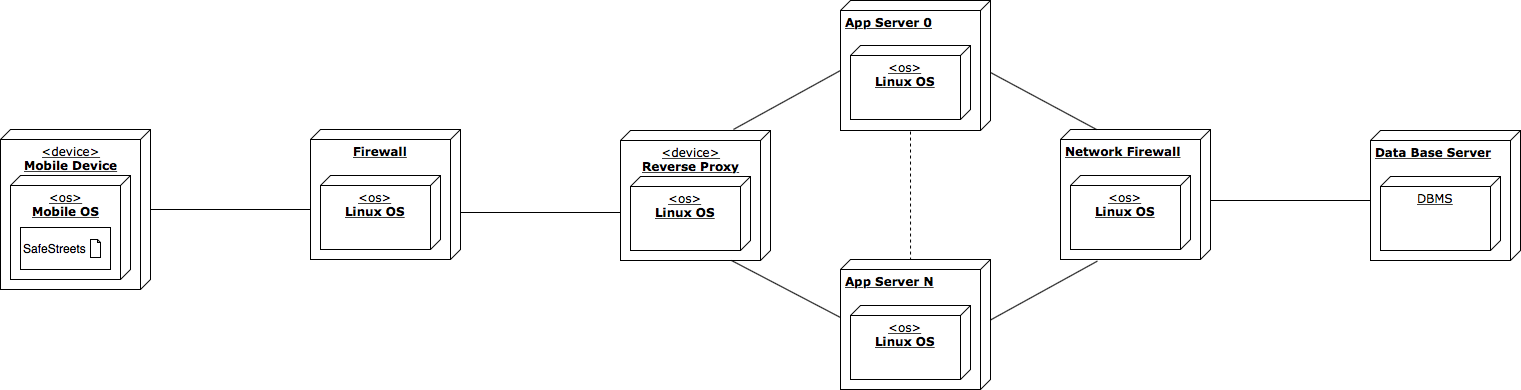
\includegraphics[scale=0.22]{Images/Diagrams/deployment_diagram.png}
			\caption{{\it SafeStreets} Deployment Diagram}
		\end{figure}
		
	The {\it System} presents a Multi-Tier architecture. The role of each node will be specified in the next section. \\ \\
			{\bf Mobile Device} \\
			It represents the Client in the architecture, hosting the {\it System}'s mobile application. This is equally valid for both {\it Users} and {\it Authorities}. \\ \\
			{\bf Firewall}\\
			It filters the access to the Reverse Proxy and is used to protect a trusted network from an untrusted network. A firewall provides protection from unauthorised requests or from malicious attacks. \\ \\
			{\bf Reverse Proxy}\\
			It retrieves resources on behalf of a client from the servers and balances the load of the various requests. It helps to achieve increased parallelism and scalability of the application. \\ \\
			{\bf Application Servers}\\
			They include all the business logic of the system, which is completely replicated to allow workload balancing. \\ \\
			{\bf Network Firewall}\\
			It does the same job of the Proxy Firewall but protecting and filtering the access to the DBMS. \\ \\
			{\bf Data Base Server}\\
			All data are stored in the Data Base Server equipped with a relational DBMS and can be retrieved with appropriate queries.
	\subsection{Runtime View}
	{\bf Account Creation Runtime View} \\
	The first sequence diagram describes the order of the events that occurs when a {\it Guest} tries to register as a {\it User} of the {\it SafeStreets} application. The actors involved in this scenario are the {\it SafeStreets}  mobile application on the Client side, while on the Server side the Authentication Manager, the User Manager and the Data Manager. The external component are the Database and the Mail Service Interfaces. \\
	The {\it Guest} selects the register button and fill the the registration form, then the request is validated, if not there's an alter. If the validation process is done correctly it's created a new {\it User}, inserted in the Database and e-mail confirmation with a code is sent to the new {\it User}.
	\begin{figure}[H]
			\centering
			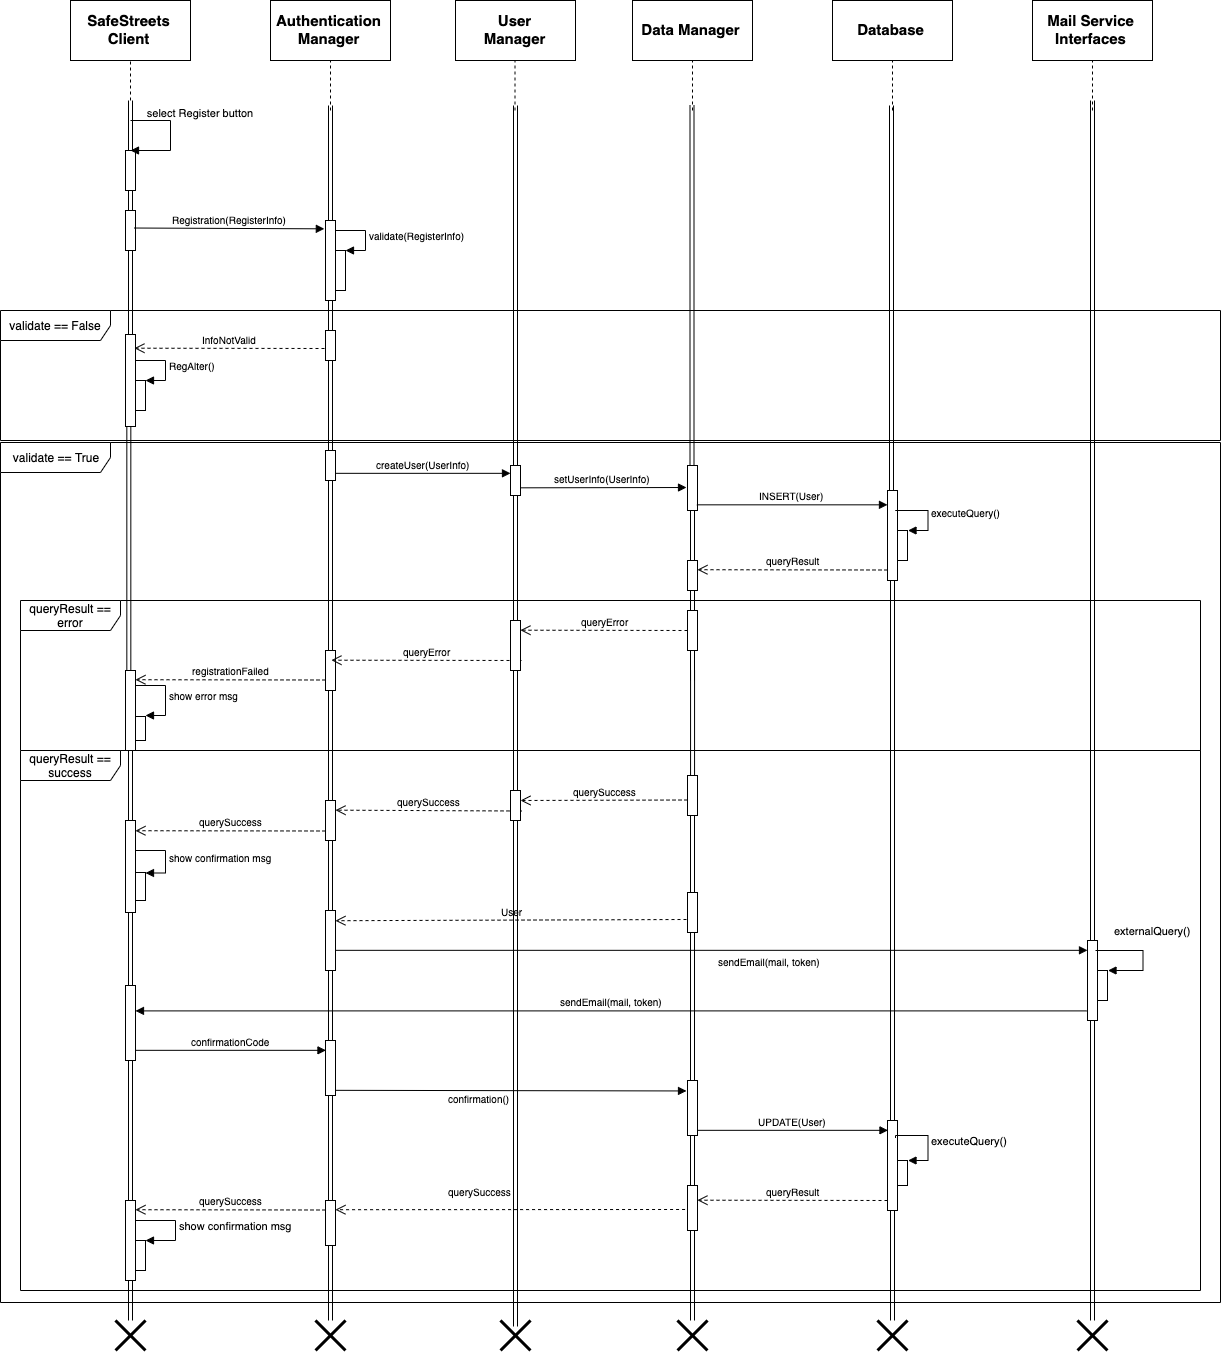
\includegraphics[scale=0.26]{Images/Diagrams/Runtime/registration_runtime.png}
			\caption{{\it SafeStreet} Account Creation Runtime View}
	\end{figure}	
	\pagebreak
	\noindent
	{\bf Log-in Runtime View} \\
	The second sequence diagram describes the order of the events that occurs when a {\it User} or {\it Authority} tries to log-in to the application. The actors involved in this scenario are the {\it SafeStreets} applitacion on the Client and on the Server side the Authentication Manager and Data Manager. The external component is the Database. \\ 
	The {\it User's} application selects the login tab and fill the the form with credentials, then the request is validated, if not there's an alter. If the validation process is done correctly it's created an access token and the {\it User} grant access to the application.
	\begin{figure}[H]
			\centering
			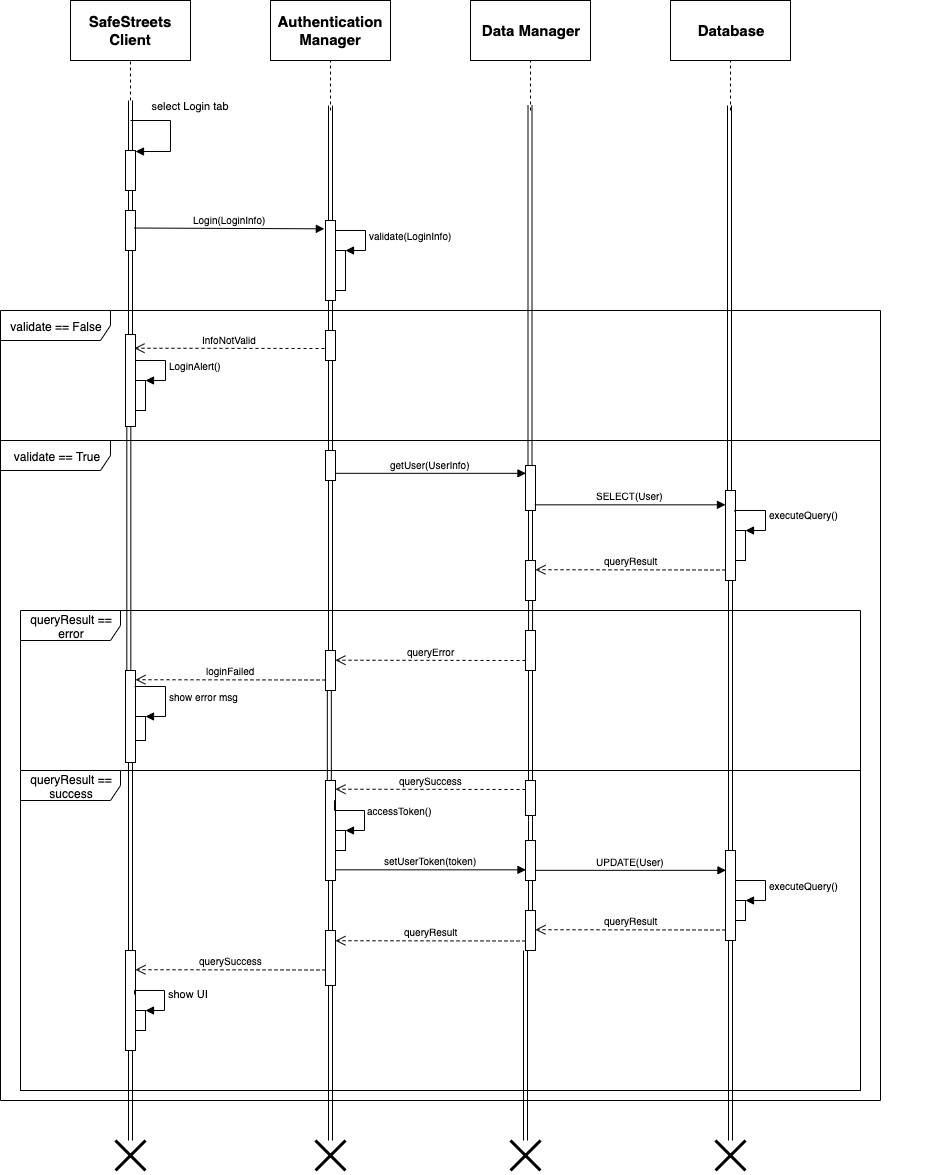
\includegraphics[scale=0.33]{Images/Diagrams/Runtime/login_runtime.png}
			\caption{{\it SafeStreets} Log-in Runtime View}
	\end{figure}
	\pagebreak
	\noindent	
	{\bf Report Violation Runtime View} \\
	The third sequence diagram describes the order of the events that occurs when a {\it User} tries to report a violation. The actors involved in this scenario are the {\it SafeStreets} application on the Client while on the Server side the Authentication Manager, Report Manager, Plate Img Controller, Data Manager. The external components are the Database, GPS Service and Notification Service Interfaces. \\ 
	The {\it User} selects the report tab, the authorisation is checked, then the {\it User} insert all the data needed for reporting the violation. Position data are retrieved from the GPS Service. Once the {\it User} has loaded the data, the image is processed by the Plate Img Controller in order to check if the image has been modified or not. If the validation process is done correctly it's created a notification in the Database, otherwise the {\it User} must re-take the photo and submit again the notification.
	\begin{figure}[H]
			\centering
			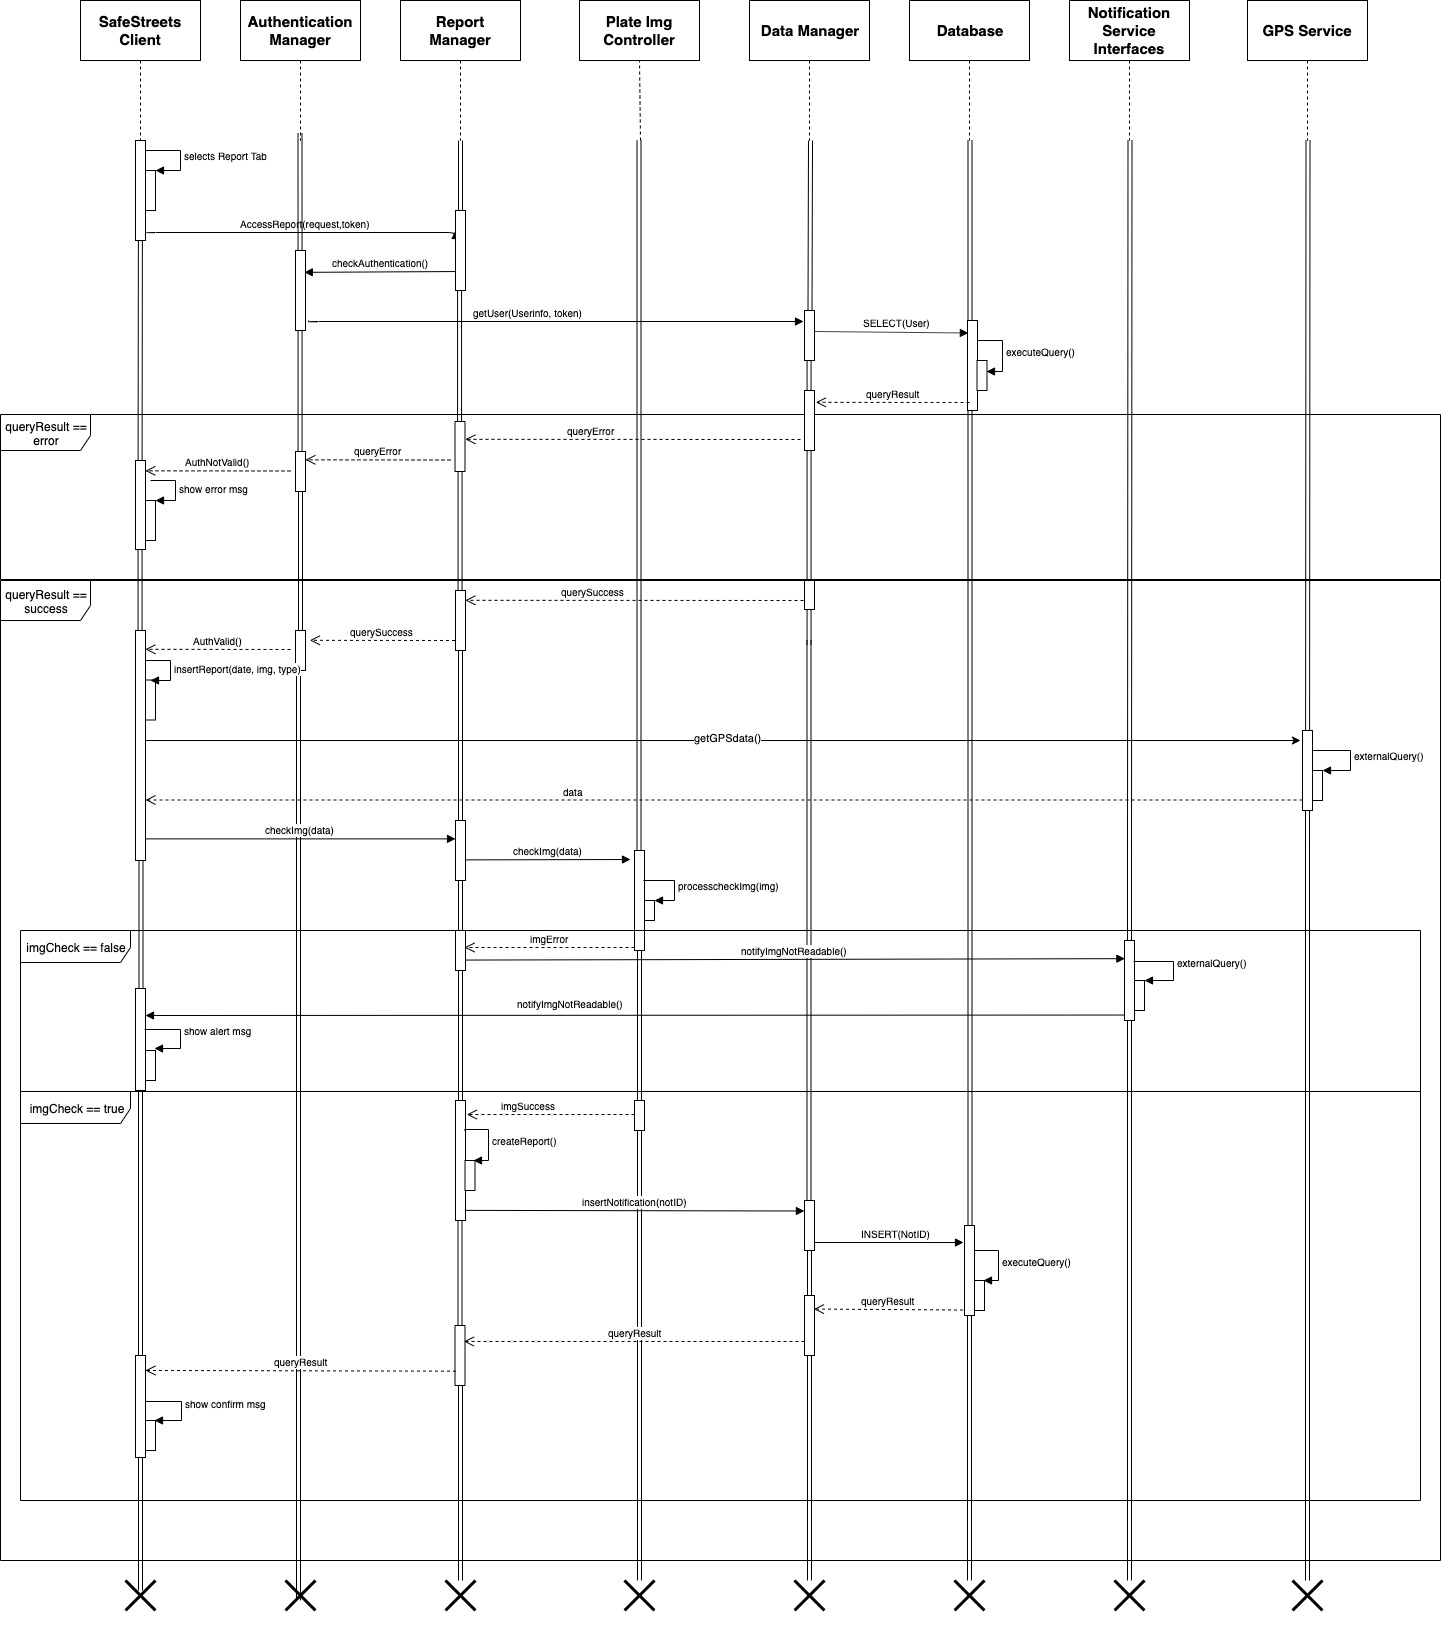
\includegraphics[scale=0.22]{Images/Diagrams/Runtime/report_runtime.png}
			\caption{{\it SafeStreets} Report Violation Runtime View}
	\end{figure}
	\pagebreak
	\noindent
	{\bf Maps Access Runtime View} \\
	The fourth sequence diagram describes the order of the events that occurs when a {\it User} or {\it Authority} tries to access Maps Statistics. The actors involved in this scenario are the {\it SafeStreets} application on the Client while on the Server side the Authentication Manager, Statistics Manager and Data Manager. The external components are the Database and Map Service Interfaces. \\ 
	The {\it User's} application selects the map tab, the authorisation is checked, then the Statistics manager get the Notification Data from the Database and the Map from the external interface. After that it computes the Map Statistics and the Client show the interface to the {\it User}, based on the visibility level, because {\it User} and {\it Authority} can see different data.
	\begin{figure}[H]
			\centering
			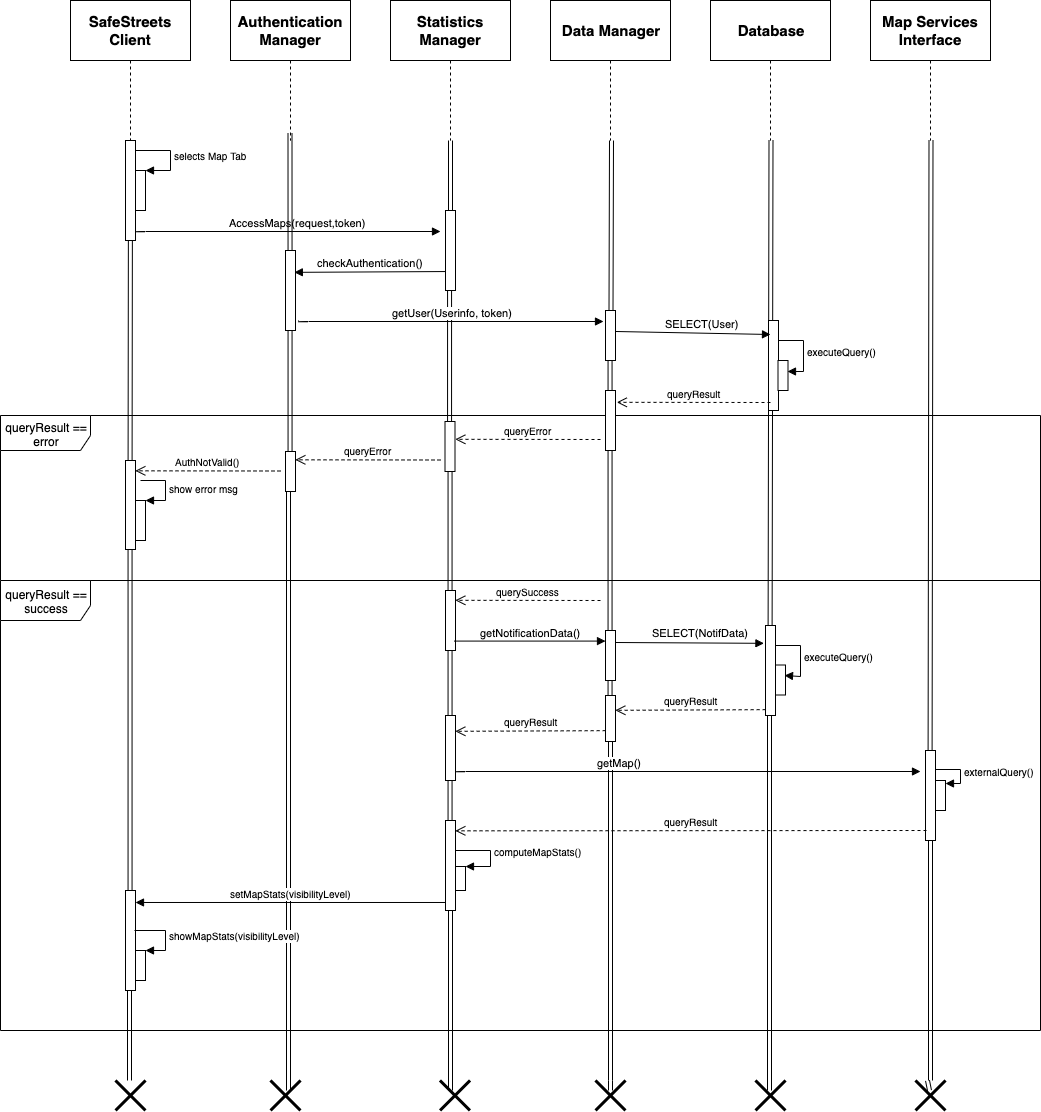
\includegraphics[scale=0.33]{Images/Diagrams/Runtime/maps_runtime.png}
			\caption{{\it SafeStreets} Maps Access Runtime View}
	\end{figure}
	\pagebreak
	\noindent
	{\bf Statistics Access Runtime View} \\
	The fifth sequence diagram describes the order of the events that occurs when a {\it User} or {\it Authority} tries to access Statistics. The actors involved in this scenario are the {\it SafeStreets} application on the Client while on the Server side the Authentication Manager, Statistics Manager and Data Manager. The external components is the Database. \\ 
	The {\it User's} application selects the Statistics tab, the authorisation is checked, then the Statistics manager get the Stats Data from the Database and computes the Statistics that must be shown to the {\it User}. Based on the different visibility level, {\it User} or {\it Authority} can see different statistics and insights generate from the notifications and/or tickets data.
	\begin{figure}[H]
			\centering
			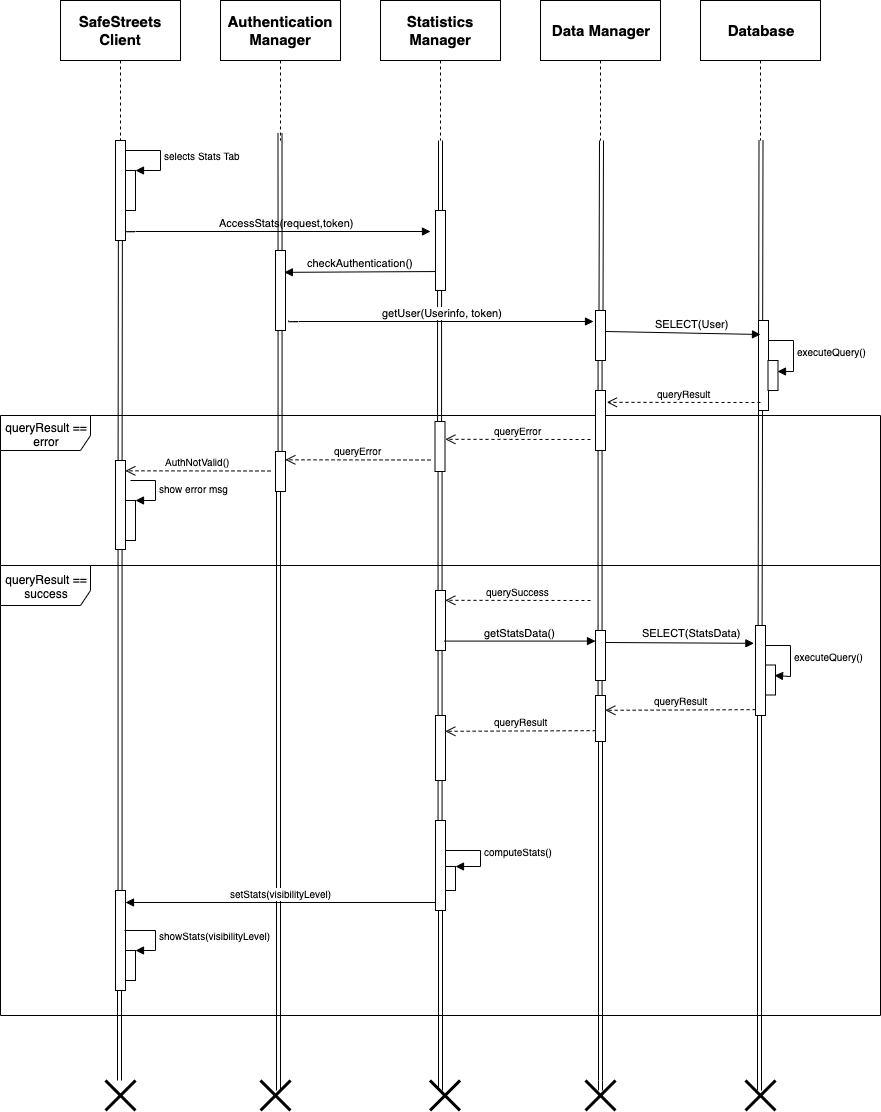
\includegraphics[scale=0.34]{Images/Diagrams/Runtime/stats_runtime.png}
			\caption{{\it SafeStreets} Statistics Access Runtime View}
	\end{figure}
	\pagebreak
	\noindent
	{\bf Ticket Generation Runtime View} \\
	The sixth sequence diagram describes the order of the events that occurs when an {\it Authority} validate or refuse the report generated from the notifications' data, that's used to generate the ticket. The actors involved in this scenario are the {\it SafeStreets} mobile application on the Client side while on the Server the Authentication Manager, Ticket Manager and Data Manager. The external component are the Database and the Municipality Service Interfaces. \\
	The {\it Authority} selects the Tickets tab, the authorisation is checked, then the Ticket Manager request the list of the notifications and show them to the User. In order to validate or refuse the ticket the {\it Authority} has to select one of them and confirm or not that is an effective violation. The Municipality has the privileges to check and generate the effective ticket based on the {\it Authority}'s validation.
	\begin{figure}[H]
			\centering
			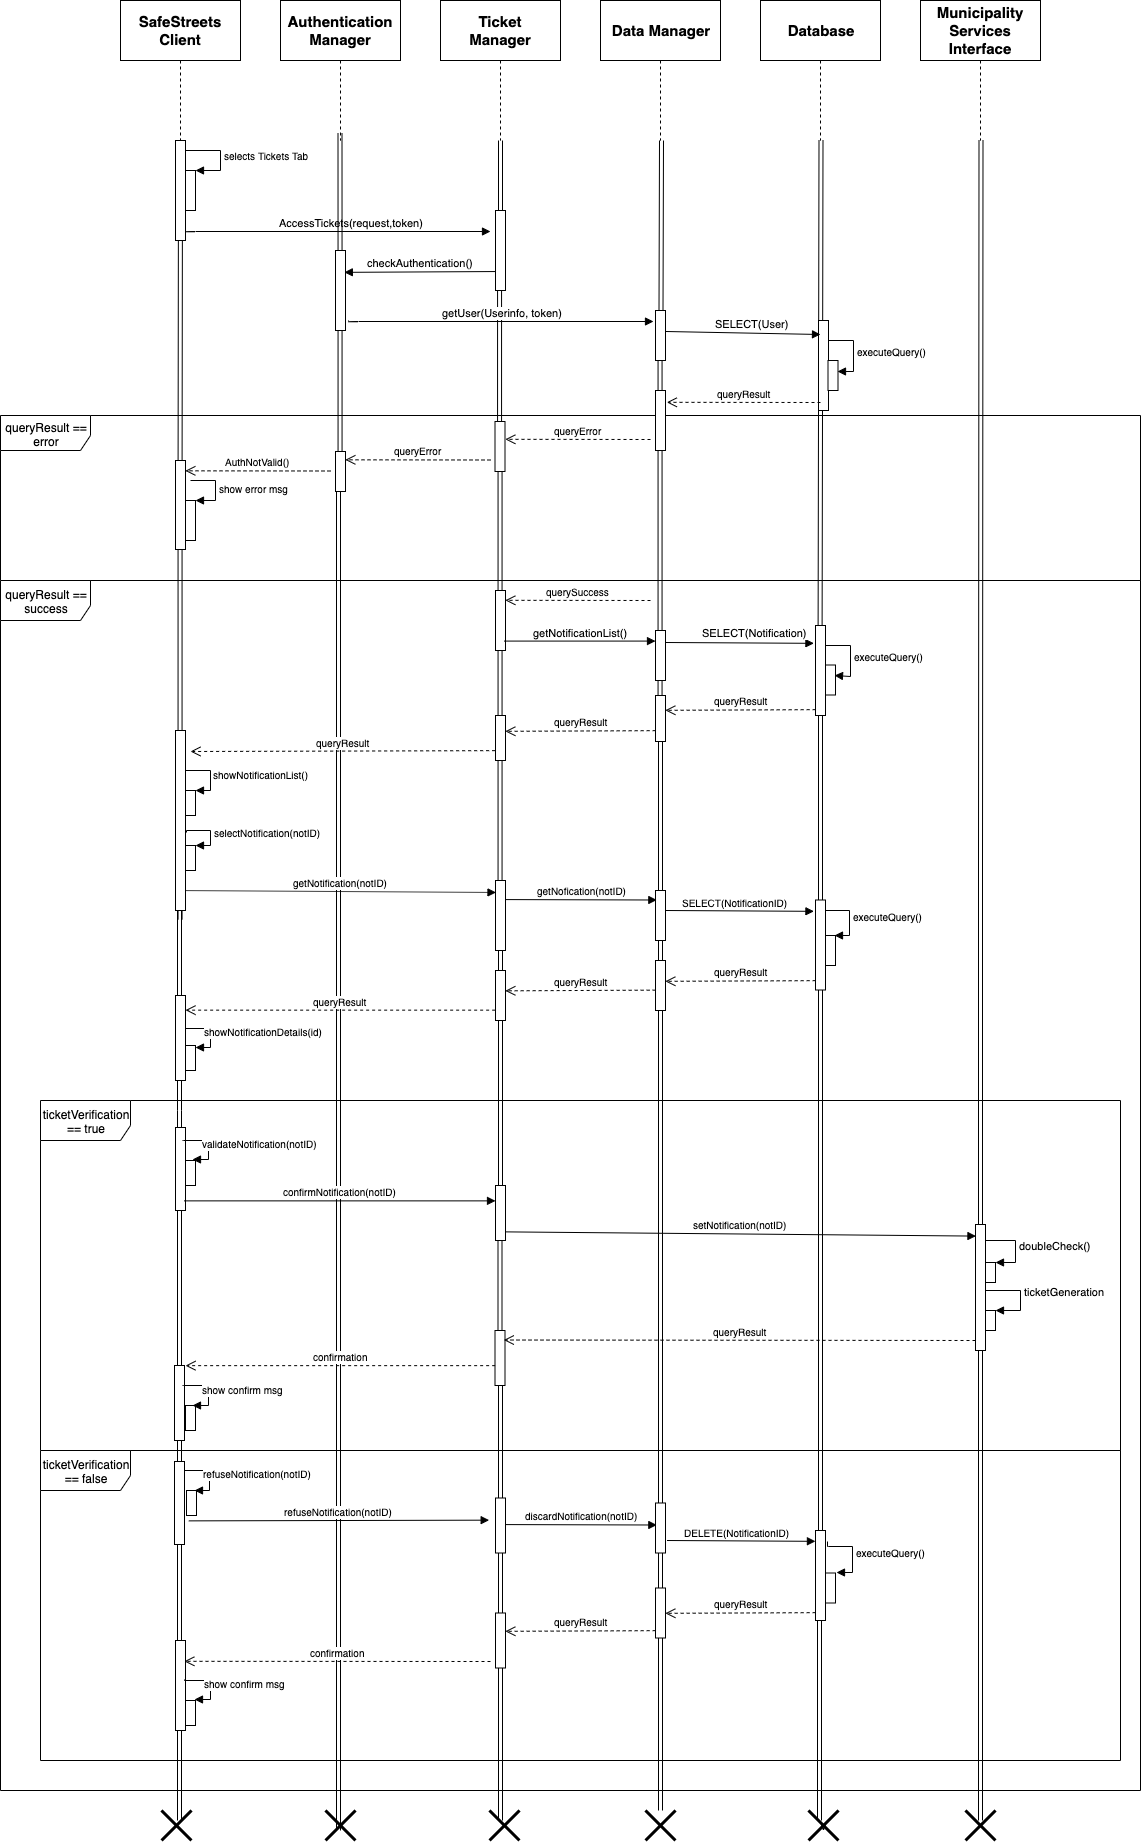
\includegraphics[scale=0.19]{Images/Diagrams/Runtime/tickets_runtime.png}
			\caption{{\it SafeStreets} Ticket Generation Runtime View}
	\end{figure}
	\pagebreak
	\noindent	
	{\bf Interventions Suggestion Runtime View} \\
	The seventh sequence diagram describes the order of the events that occurs when a list of intervention is suggested to the {\it Authority} and he/she can confirm the solution as feasible or not. The actors involved in this scenario are the {\it SafeStreets} mobile application on the Client side while on the Server the Authentication Manager, Intervention Manager and Data Manager. The external component are the Database and the Municipality Service Interfaces. \\
	The {\it Authority} selects the Interventions tab, the authorisation is checked, then the Intervention Manager request the intervention data from the Database showing the list of the suggestions to the {\it Authority} that has the task to confirm one or more of them as feasible or not. Then the confirmation is sent to the Municipality that can starts the procedure to solve the issue.  
	\begin{figure}[H]
			\centering
			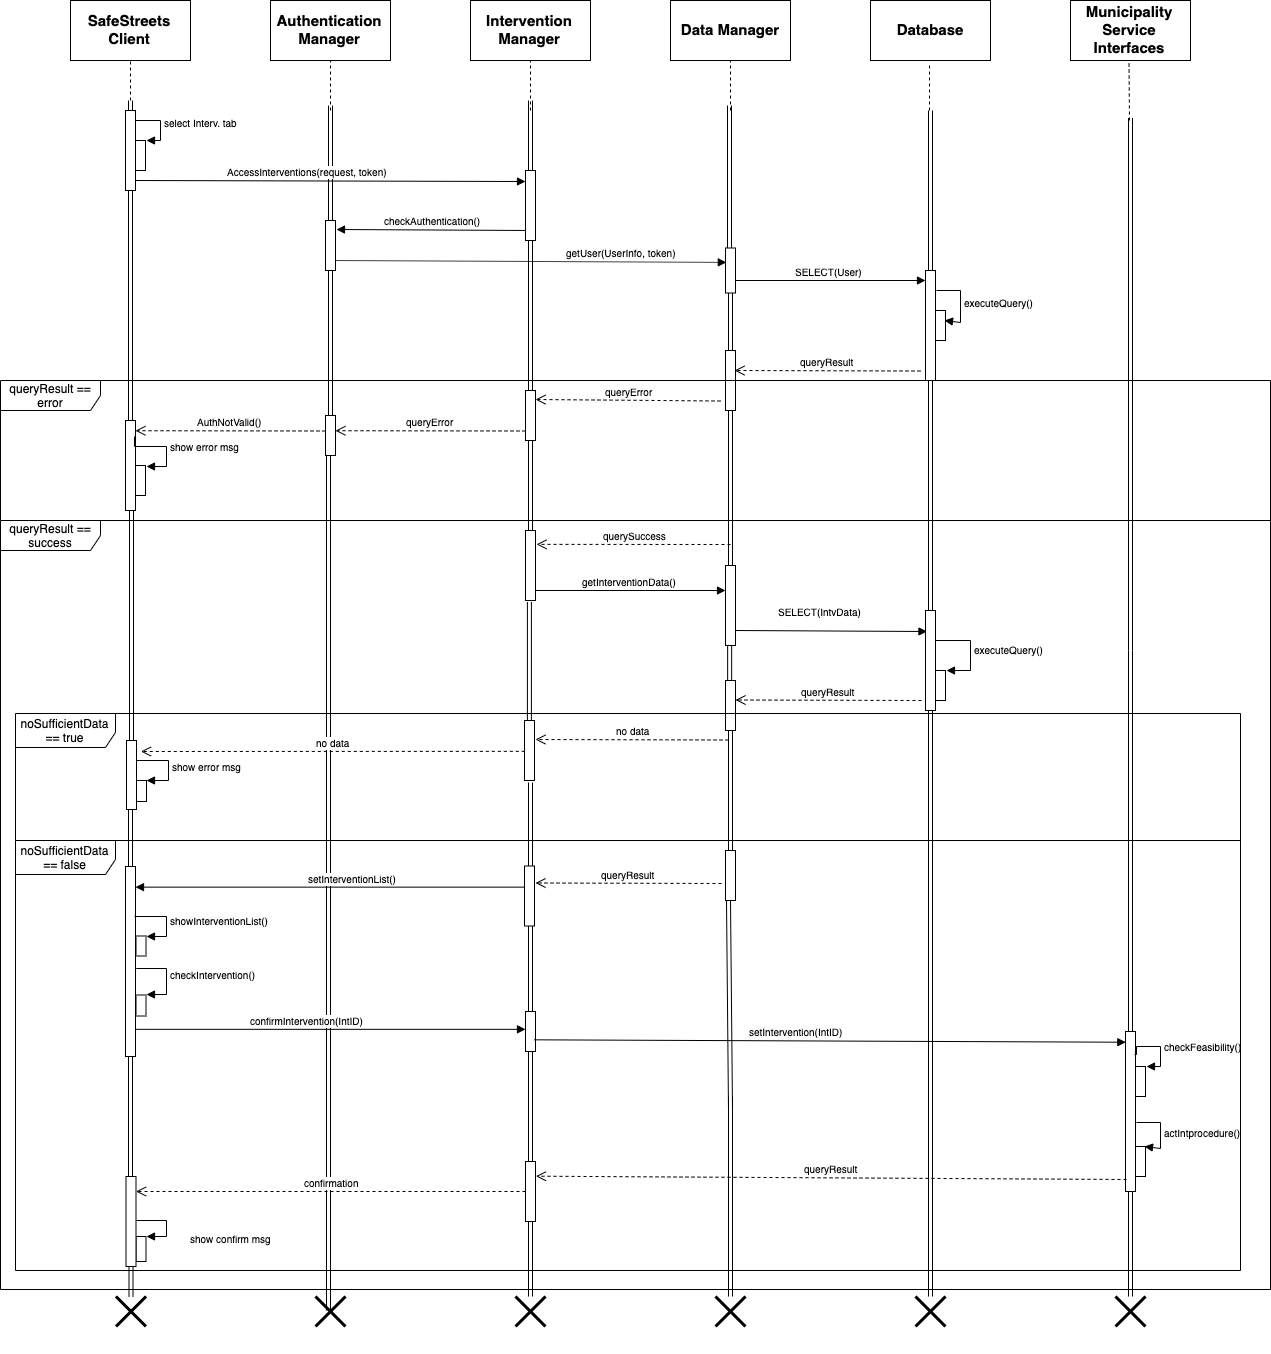
\includegraphics[scale=0.30]{Images/Diagrams/Runtime/interventions_runtime.png}
			\caption{{\it SafeStreets} Interventions Suggestion Runtime View}
	\end{figure}
	\pagebreak
	\noindent
	\subsection{Component Interfaces}
	{\bf Interface Diagram} \\
	The diagram below represents the Component View of the {\it System}, with methods that have been shown in the Runtime View. Some self calls are omitted. 
		\begin{figure}[H]
			\centering
			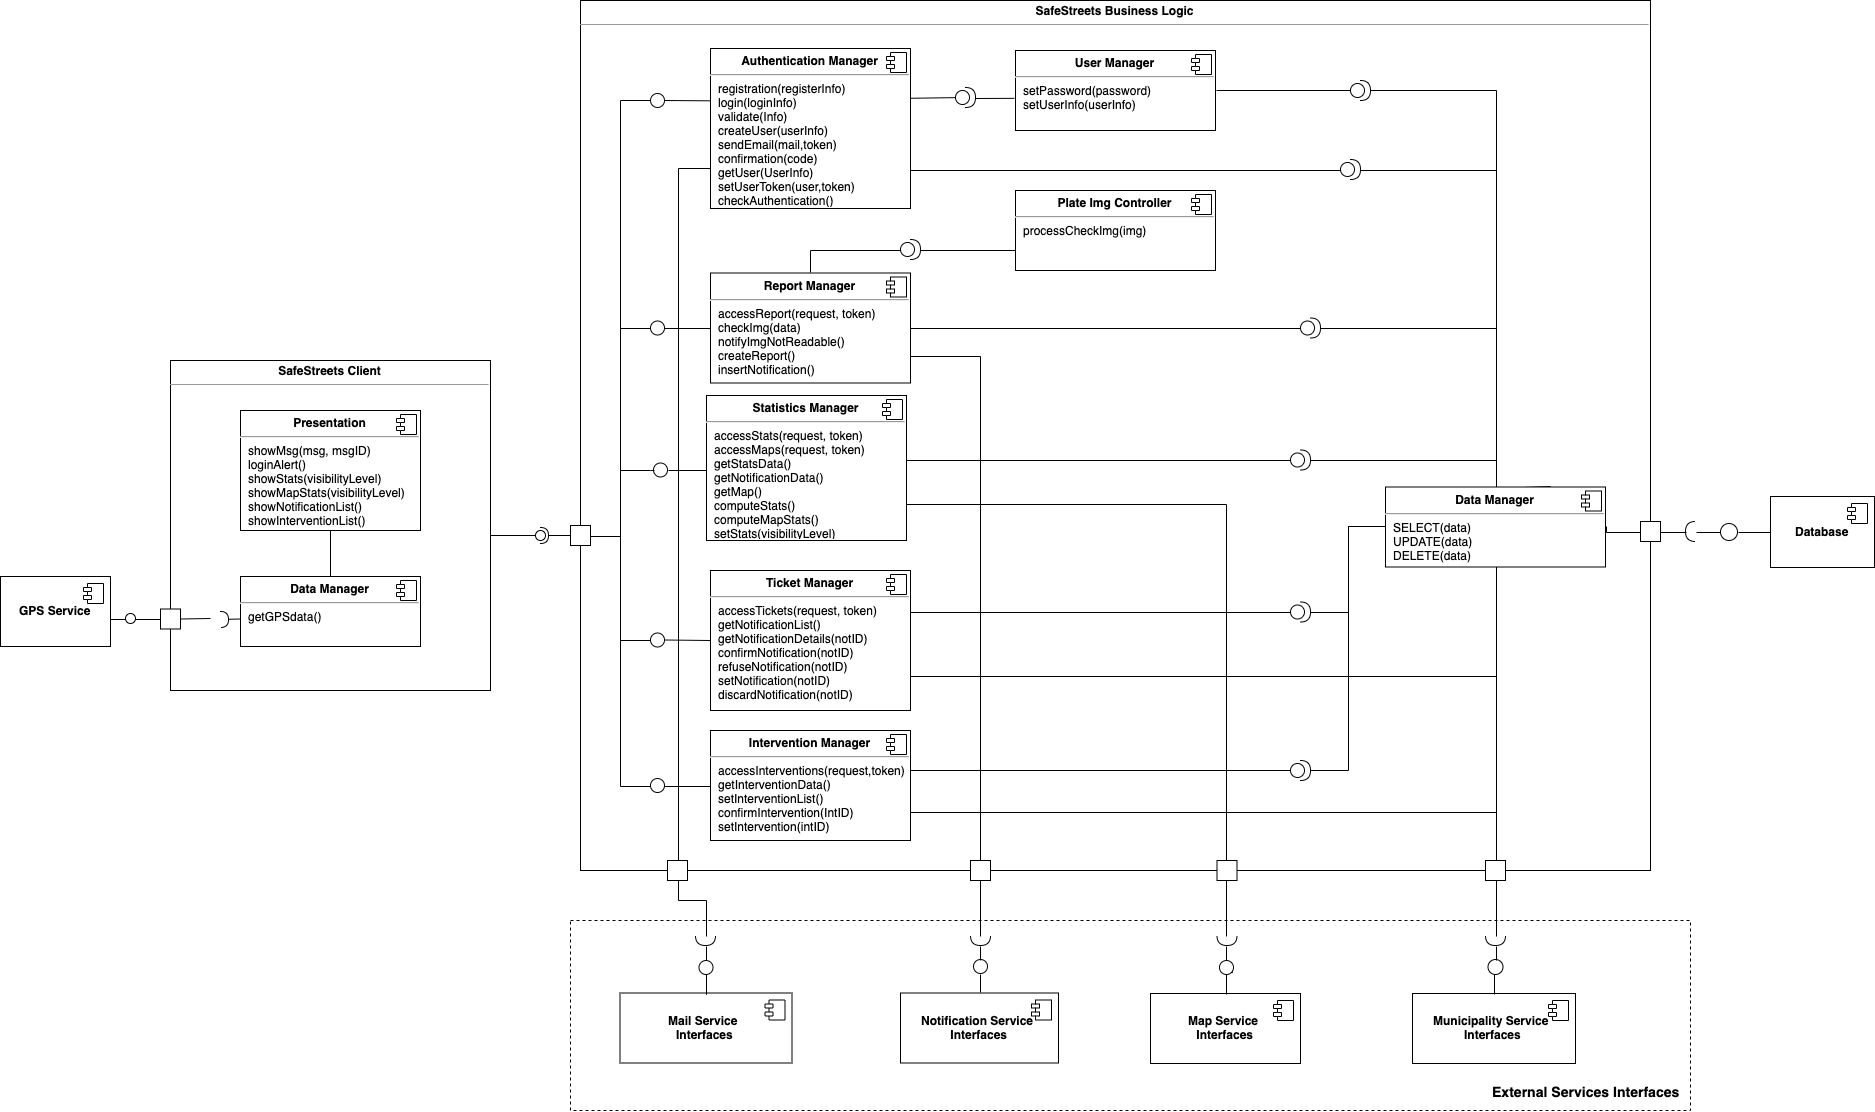
\includegraphics[scale=0.20]{Images/Diagrams/interface_diagram.png}
			\caption{Component Interface Diagram}
		\end{figure}	
	\noindent
	{\bf SafeStreets Client} 
	\\ 
	In this section we will describe all the methods of the Client, in particular related to the Presentation layer.
	\begin{itemize}
		\item {\bf Presentation}
		\begin{itemize}
		\item {\it showMsg(msg, msgID)}: this method has to show the alert or confirmation messages to the {\it User}, using as parameter the type of message and the different id on the basis of the case that has been taken into account. 
		\item {\it loginAlert()}: display the alert when the Authentication Manager does not validate the credentials entered to access the application.
		\item {\it showStats(visibilityLevel)}: display the statistics generated from the notifications' data and tickets' data based on the visibilityLevel of User or Authority.
		\item {\it showMapStats(visibilityLevel)}: display the statistics on the map generated from the data based on the visibilityLevel of User or Authority, for showing sensitive information.
		\item {\it showNotificationList()}: display to the Authority the list of tickets that can be validated or refused.
		\item {\it showInterventionList()}: display the intervention list suggested by the System to the Authority.
		\end{itemize} 
		\item {\bf Data Manager}
		\begin{itemize}
		\item {\it getGPSData()}: get the coordinates data in order to retrieve the position of the physical device.
		\end{itemize}
	\end{itemize} 
	{\bf SafeStreets Business Logic} \\
	In this section we will describe the methods of the Business Logic, divided per each component.
	\begin{itemize}
    	\item {\bf Authentication Manager}
       		\begin{itemize}
        		\item {\it registration(registerInfo)}: method that processes the registration using the information filled by the Guest.
        		\item {\it login(loginInfo)}: method that processes the login using the information filled by the User or Authority.
        		\item {\it validate(Info)}: method that validate the authorisation of the User's application to use the functionalities of the application.
        		\item {\it createUser(userInfo)}: method that create a new User using the information filled by the Guest in the form, if the process has been done correctly.
        		\item {\it sendEmail(mail, token)}: method that invoke the external service to send the confirmation e-mail to the new User.
        		\item {\it confirmation(code)}: method used to confirm an action.
        		\item {\it getUser(userInfo)}: method that retrieve information about privileges of the User/Authority starting from his/her information.
        		\item {\it setUserToken(user, token)}: method that set a token for the User/Authority.
        		\item {\it checkAuthentication()}: method that process a check to be sure that the User has the authorisation to proceed with the use of the application. 
    		\end{itemize}
    	\item {\bf User Manager}
    		\begin{itemize}
        		\item {\it setPassword(password)}: method that set the password for the User's application.
        		\item {\it setUserInfo(userInfo)}: method that sets the information for the User's application.
    		\end{itemize}
    	\item {\bf Report Manager}
    		\begin{itemize}
        		\item {\it accessReport(request, token)}: method invoked to access the report function of the application.
        		\item {\it checkImg(data)}: method that start the process of image checking.
        		\item {\it notifyImgNotReadable()}: method that invoke the external Notification Service to alert the user to re-enter the image of the violation because it's not readable.
        		\item {\it createReport()}: method that create the effective report with all the information provided by the User in the notification. 
        		\item {\it insertNotification()}: method invoked to memorise the notification if the process has been done correctly.
    		\end{itemize}
    	\item {\bf Plate Img Controller}
    		\begin{itemize}
        		\item {\it processCheckImg(img)}: method that using as input the image of the violation, analyse the image and determine if it has been modified or not, and if that's readable or not.  
        	\end{itemize}
    	\item {\bf Statistics Manager}
    		\begin{itemize}
        		\item {\it accessStats(request, token)}: method invoked to access the statistics function of the application.
        		\item {\it accessMaps(request, token)}: method invoked to access the maps function of the application.
        		\item {\it getStatsData()}: method that get all the data needed for the statistics generation.
        		\item {\it getNotificationData()}: method that get all the data generated from the Users' notification.
        		\item {\it getMap()}: method that invoke the external Map Service to cross the data with the map visualisation.
        		\item {\it computeStats()}: method that compute the Statistics to show the User or Authority.
        		\item {\it computeMapStats()}: method that compute the Map Statistics to show the User or Authority.
        		\item {\it setStats(visibilityLevel)}: method that set the Statistics to show to the User or Authority, based on the visibility level. 
    		\end{itemize}
    	\item {\bf Ticket Manager}
    		\begin{itemize}
        		\item {\it accessTickets(request, token)}: method invoked to access the tickets function of the application
        		\item {\it getNotificationList()}: method that get all the notification list to show to the User
        		\item {\it getNotificationDetails(notID)}: method that get the information about a specific notification based on the notID.
        		\item {\it confirmNotification(notID)}: method invoked when a notification is confirmed by the Authority, based on the notID.
        		\item {\it refuseNotification(notID)}: method invoked when a notification is refused by the Authority, based on the notID.
        		\item {\it setNotification(notID)}: method that invoke the external Municipality Service to set the notification in the list of the feasible one, so the process of ticket generation can be done.
        		\item {\it discardNotification(notID)}: method that discard the notification after it has been refused, based on the notID.
    		\end{itemize}
    	\item {\bf Intervention Manager}
    		\begin{itemize}
        		\item {\it accessInterventions(request, token)}: method invoked to access the intervention function of the application.
        		\item {\it getInterventionData()}: method that get all the data needed for the interventions suggestion function.
        		\item {\it setInterventionList()}: method that set the intervention list to show to the User. 
        		\item {\it confirmIntervention(intID)}: method invoked when the Authority confirm that the intervention is feasible based on the ID of the intervention.
        		\item {\it setIntervention(intID)}: method that invoke the external Municipality Service to set the Intervention in the list of the feasible one, in order to start the phase before the physical intervention, based on the notification ID.  
    		\end{itemize}
    	\item {\bf Data Manager}
    		\begin{itemize}
        		\item {\it SELECT(data)}: method that select the data as input from the external database service.
        		\item {\it UPDATE(data)}: method that update the data as input from the external database service.
        		\item {\it DELETE(data)}: method that delete the data as input from the external database service.
        		\item {\it INSERT(data)}: method that insert the data as input from the external database service.
    		\end{itemize}
	\end{itemize}
	
	\pagebreak
	
	\subsection{Selected Architectural Styles and Patterns}
	{\bf Multi-tier Architecture} \\
	As stated in the Overview section, the {\it System}'s architecture is a multi-tier \mbox{architecture}. A multi-tier architecture is a client-server architecture where presentation, application logic, and data management functions are physically separated. This division let each tier perform specific tasks, avoid the dependancy from a single node for all the architecture and facilitates the modification of a single tier. This guarantees a better maintenance of {\it System}. \\ \\
	{\it SafeStreets} implements a three-tier architecture, with the following layer: Presentation tier, Business (or Domain) logic tier and Data management tier. We'll now analyse each one in details:
	\begin{itemize}
		\item {\bf Presentation tier:} this is the top level of the application; this tier is completely managed by the Client device, which is a mobile application, both for {\it Users} and {\it Authorities}. The main task is to display to the User's application all the information provided by the Application Server, thanks to the GUI of the mobile device. It also displays also the information of the external services. This is the only tier directly accessible from the User's application. 
		\item {\bf Business Logic tier:} this tier host the Application Servers of {\it SafeStreets}. As explained by the name it implements the Business/Domain logic layer and not the storage. The deployment is done by replicating each server as many times as necessary to guarantee the non-functional requirements. Also, each one of the server is stateless. In case of many request, it's possible to add more machines to handle the traffic rise. It controls all the application functionality with all his processing. This tier contains the reverse proxy.		
		\item {\bf Data management tier:} this tier is represented by the Database. A cloud solution is adopted in order to eliminate from the {\it System} tasks like the reliability and management of the physical database. So, it implements the data access layer and encapsulate all the related mechanisms.  
	\end{itemize}
	{\bf Thin Client} \\
	The thin client paradigm is implemented for the interaction between the physical device machine and the {\it System}. A thin client needs to perform few computation, very close to no computation, but it has to handle the communication. The main advantage of this architecture is that it’s easier to keep data synchronised across multiple clients. It also requires less effort to create new client implementation because there's no logic. A thin client does not rely on local storage since all the business logic is on the application servers, which have enough computing power. Even if our Client implementation has a Data Manager and it's used to retrieve the GPS data because the contribution to the data access is very low, we consider the Client tier as a Thin Client, which host the Presentation layer.
	\\ \\
	{\bf MVC} \\
	The {\it System} architecture follow the MVC (Model-View-Controller) pattern. This pattern of functionality separation has numerous advantages like simultaneous development, high cohesion and loose coupling between classes, multiple views for the model and ease of modification. It's considered a best practice in the development process and respect the fundamental design principles of software engineering.
	\begin{itemize}
		\item {\bf Model}: that's everything related to the application's data and integrity. It's implemented in our {\it System} by the external database.
		\item {\bf View}: this corresponds to the Presentation tier, that's the only interface between the User's application and the {\it System}.
		\item {\bf Controller}: that's responsible for the application logic. In our case is stateless and replicable and corresponds to the business logic layer of the {\it System}.
	\end{itemize}
		
	\subsection{Other Design Decisions}
	{\bf Database} \\
	It's used a relational model for the {\it SafeStreets} database because it's considered the  right schema for the purpose of our {\it System}. Even if the {\it System} has to compute a lot of calculation, the majority of the operations needs to select small amount of data; these are repetitive operations that should be computed fast, so the chose of a non-relation model is not take into account. Also, a relation model could be accessed using SQL that's a standard across the industry, instead of using a specific language that a non-relational database needs.
	\\ \\ 
	{\bf Firewall} \\ 
	The {\it System} architecture has two firewalls that guarantee a separation between the mobile device and the reverse proxy and between the application server and the database. There's an application proxy that provide one of the most secure types of access you can have in a security gateway, in fact every time an application makes a request, the application intercepts the request to the destination system. There's also a network firewall that filters the packets trying to pass through them, keeping the application safe.
	\\ \\
	
\pagebreak

% User Interface Design - Section 3
\section{User Interface Design}
In the section 3.1 of the RASD document are explained in details all the User Interfaces and their design. So, for further information about the UI Design, refers to the RASD document. \\
In this section is provided an overview of the UX Application flow, using the UI mockups of the RASD. It's explained the flow of the application from the point of view of the {\it User} and from the point of view of the {\it Authorities}.
	\begin{figure}[H]
			\centering
			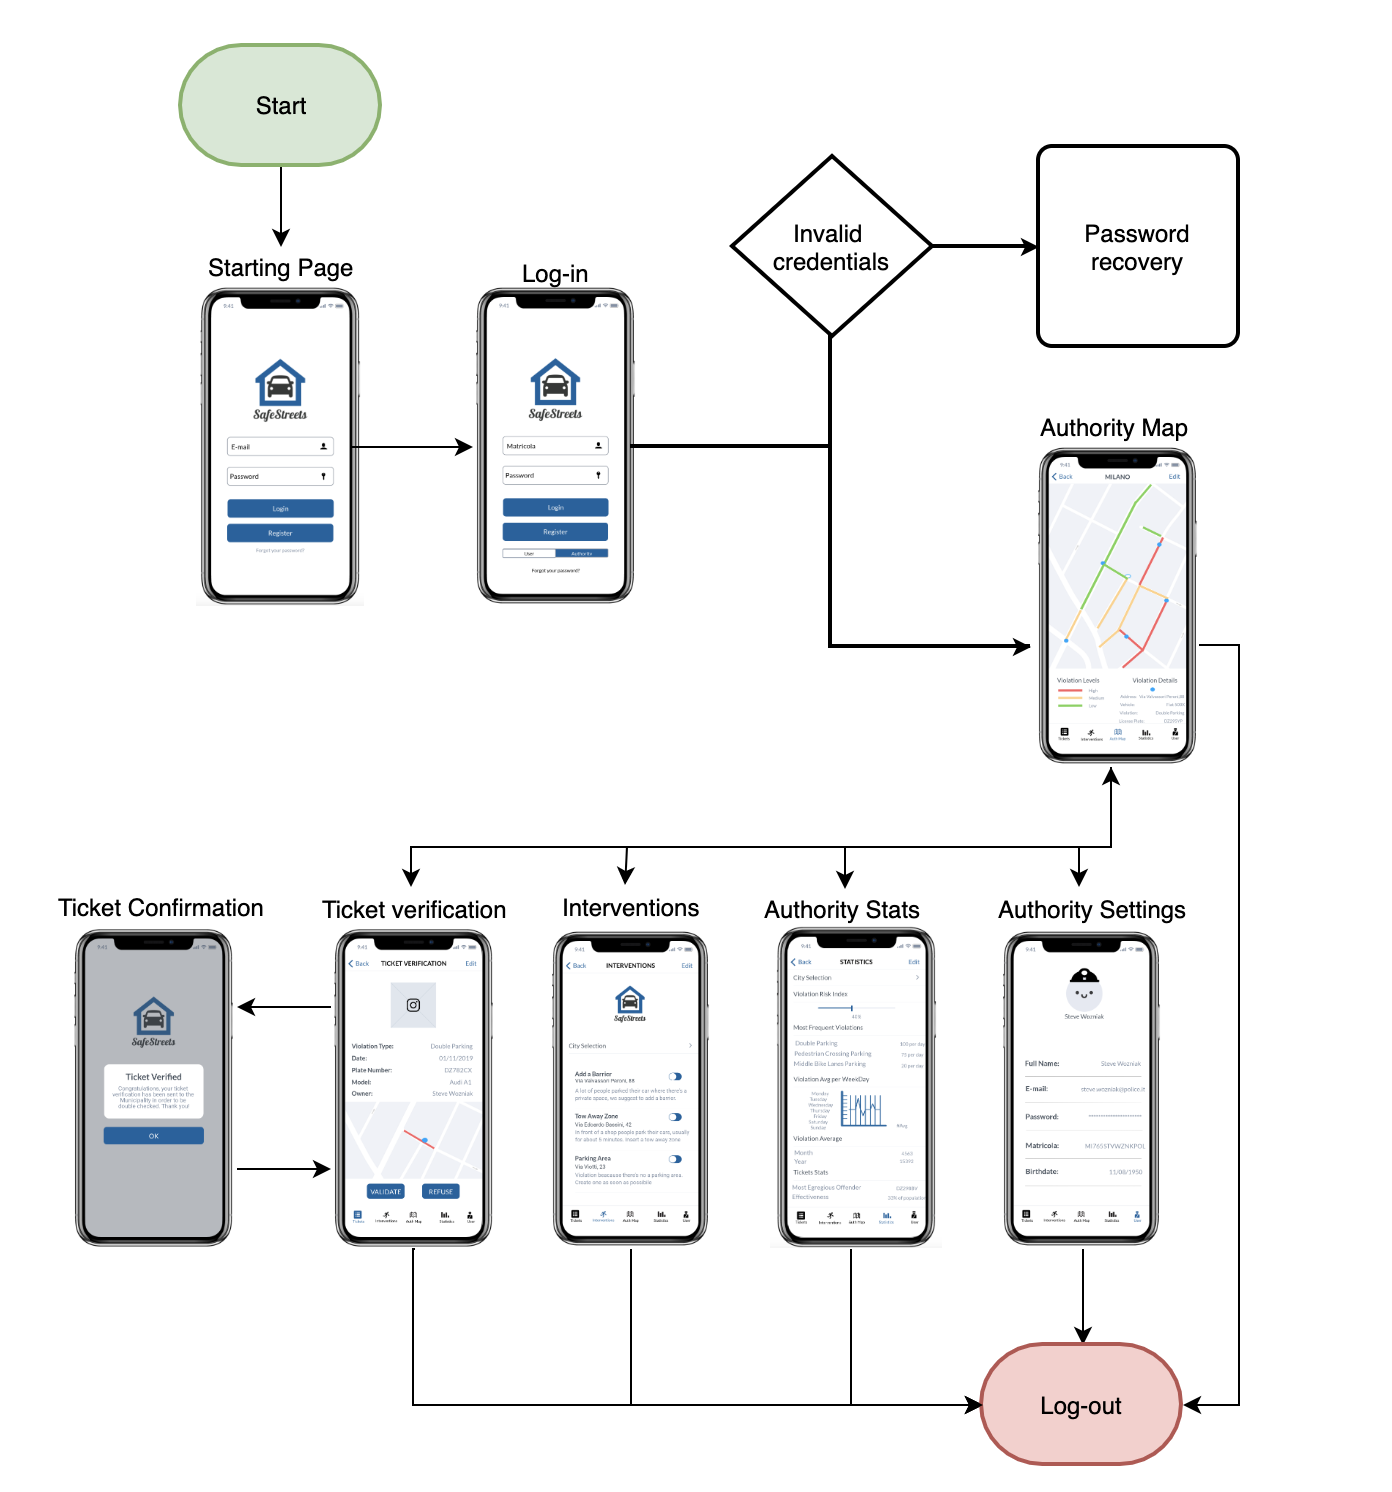
\includegraphics[scale=0.5]{Images/UX/user_ux_flow.png}
			\caption{{\it SafeStreets} User UX flow diagram}
	\end{figure}
	\begin{figure}[H]
			\centering
			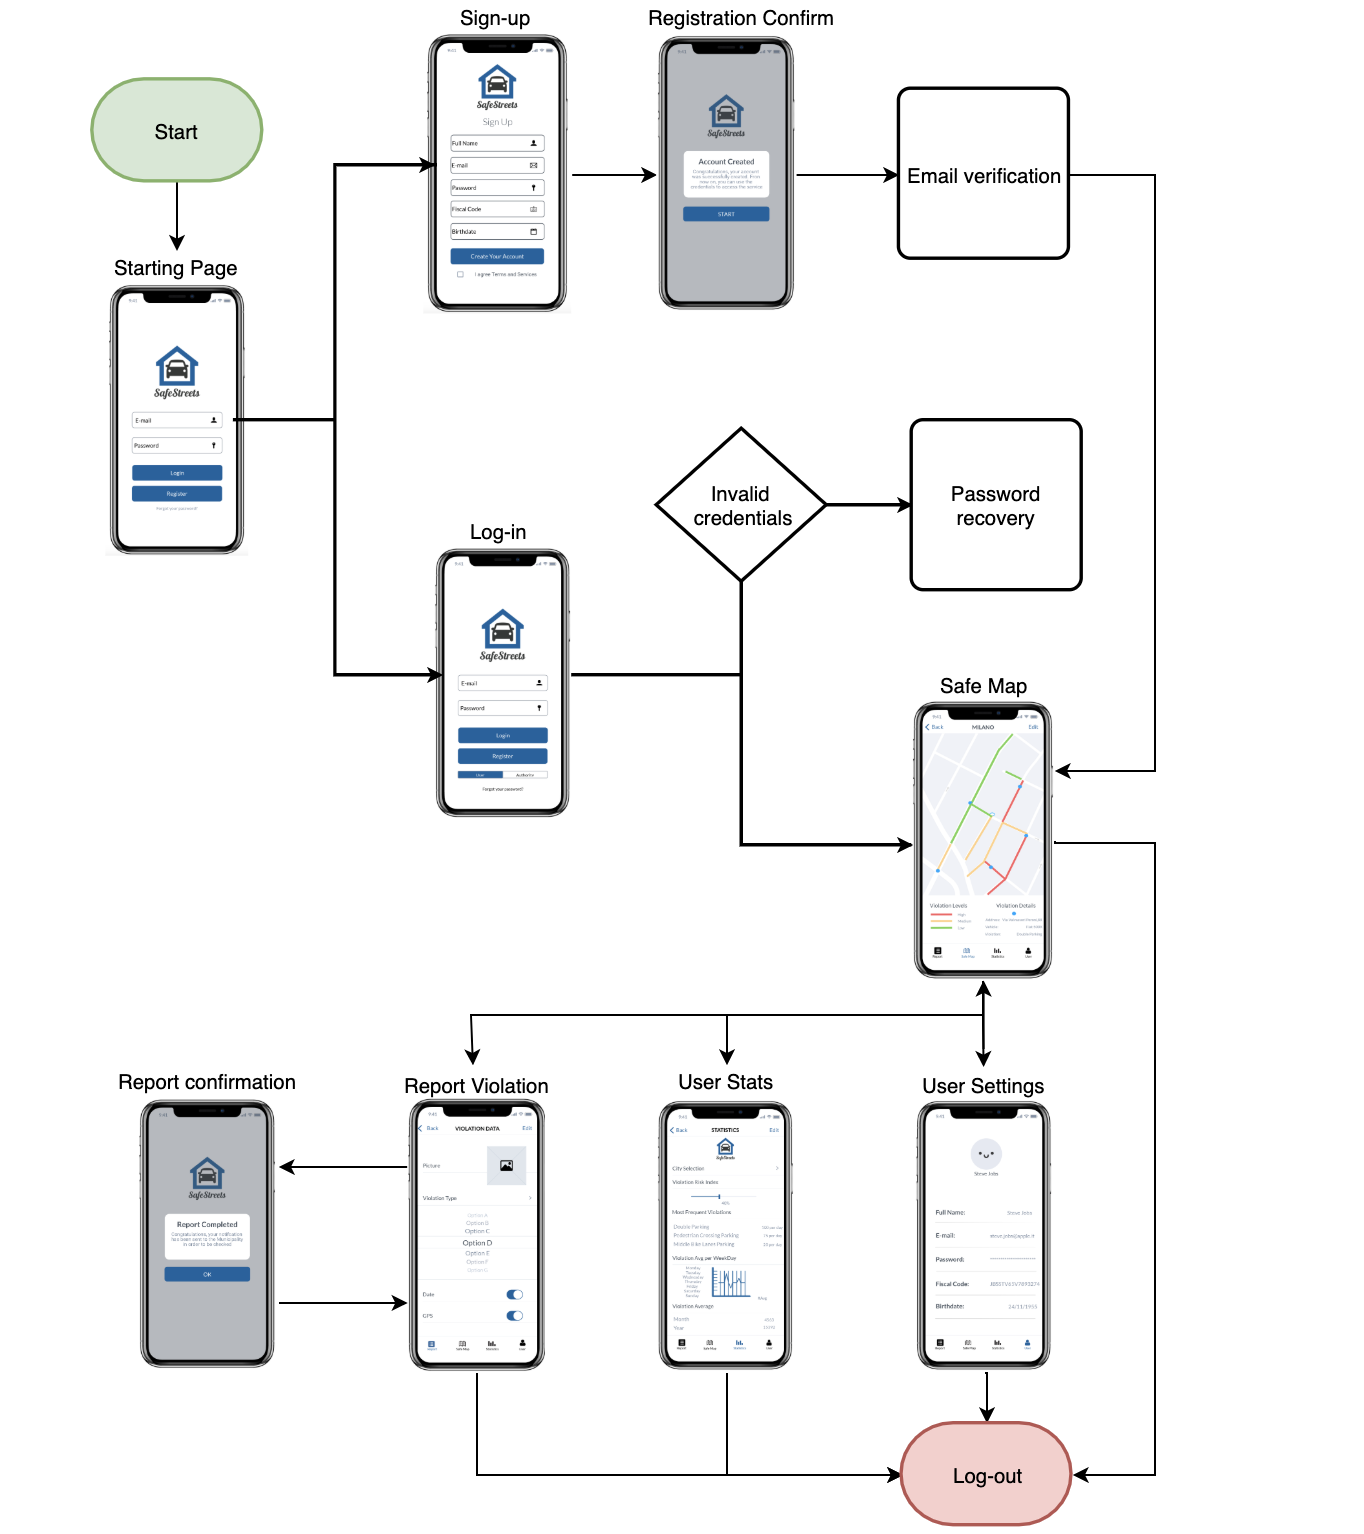
\includegraphics[scale=0.5]{Images/UX/authority_ux_flow.png}
			\caption{{\it SafeStreets} Authority UX flow diagram}
	\end{figure}

\pagebreak

% Requirements Traceability - Section 4
\section{Requirements Traceability}
	
	\begin{longtable}{| p{5 cm} | p{8 cm} |} \hline
		Component (DD) & Requirements (RASD)  \\ \hline
		\newline Data Manager (Client) & 
		\begin{itemize}
			\item {{\bf[R13]} Metadata, such as date and time, must be automatically re- trieved from the device.}
		\end{itemize}	\\ \hline
		\newline Authentication Manager & 
		\begin{itemize}
			\item  {{\bf[R1]} The System allows account to be created as a simple User or Authority.}
			\item  {{\bf [R2]} A User account can be created if the User provides the correct data: unique email and fiscal code.}
			\item  {{\bf [R4]} Users and Authority can access the service if they log-in with their credentials.}
			\item  {{\bf [R5]} The System must be able to check if the credentials are valid.
}
			\item  {{\bf [R9]} Only User with an account can create and send a report.}
		\end{itemize}		\\	 \hline	
		\newline User Manager  & 
		\begin{itemize}
			\item  {{\bf [R6]} The System must store all User credentials.}

		\end{itemize}		\\	 \hline	
		\newline Report Manager  & 
		\begin{itemize}
			\item  {{\bf [R8]} The System gives a feedback to the User if the report process is done correctly.}
			\item  {{\bf [R9]} Only User with an account can create and send a report.}
			\item  {{\bf [R10]} The System must allow the User to take a picture of the violation.}
			\item  {{\bf [R12]} The System must allow the User to select the violation type.}
			\item  {{\bf[R14]} The System must allow the User to edit information before sending the report.}
		\end{itemize}		\\	 \hline	
		\newline Plate Image Controller & 
		\begin{itemize}
			\item  {{\bf[R7]} The System must be able to analyse the picture and recognise
the plate number.
}
			\item  {{\bf [R8]} The System gives a feedback to the User if the report process is done correctly.} 
			\item  {{\bf [R11]} The System can accept or refuse the image loaded from the User.}
		\end{itemize}		\\	 \hline	
		\newline Statistics Manager & 
		\begin{itemize}
			\item  {{\bf [R18]} The System must allow the User to visualise statistics derived from the data.}
			\item  {{\bf [R29]} The System must allow the Authority to visualise statistics derived from tickets’ data.}
		\end{itemize}		\\	 \hline		
			\newline Ticket Manager & 
		\begin{itemize}
			\item  {{\bf [R23]} The System must allow the Authority to access information
about the violation notification.}
			\item  {{\bf [R24]} The System must allow the Authority to validate a ticket.}
			\item  {{\bf [R25]} The System must allow the Authority to access sensible data
about the violation.}
			\item  {{\bf [R26]} The System must advise the Authority that the violation de- tails process is done correctly.}
		\end{itemize}		\\	 \hline	
			\newline Intervention Manager & 
		\begin{itemize}
			\item  {{\bf [R20]} The System must be able to identify viability issues based on data.}
			\item  {{\bf [R21]} The System must suggest solution to address viability issue.}
			\item  {{\bf [R22]} The System must allow the Authority to access the list of possible interventions.
}
			\item  {{\bf [R23B]} The System must allow the Authority to establish if the inter- vention is feasible solutions or not.}
		\end{itemize}		\\	 \hline	
			\newline Data Manager & 
		\begin{itemize}
			\item {{\bf [R6]} The System must store all User credentials.}

			\item  {{\bf [R15]} The System must be able to store all the notifications’ data.}
			\item   {{\bf [R27]} The System must be able to store all the tickets’ data.}
		\end{itemize}		\\	 \hline			
		\caption{Requirements Traceability}	
		
	\end{longtable}
	
	\pagebreak
	
	
% Testing - Section 5
\section{Implementation, Integration and Test Plan}
	\subsection{Overview}
	The {\it System} is divided in many components, that can be divided in the following sub-systems:
	\begin{itemize}
		\item {\it Front-end Components}: this is Client application subsystem, containing the presentation and the data manager components.
		\item {\it Back-end Components}: this is the Business Logic subsystem with all its components that interacts with the database. 
		\item {\it External Components}: this are the external components that interacts with the {\it System}, such as the Map and GPS services.  
	\end{itemize}
	The strategy used to design the {\it System} was {\it Top-Down}, defining the sub-systems described above at a high-level, then refining and detailing them with all the details needed.\\
	The implementation and testing approach will follow a combination of both {\it Top-Down} and {\it Bottom-Up} strategies because it's the most reasonable choice for relatively small components and sub-systems. \\ 
	In the following paragraphs it will be presented the order of the implementation and of the integration testing between components.
		
	\subsection{Implementation}
	The implementation of the different components will be parallelised in order to divide the work between developers and for speeding up the implementation process. \\
	The order of the implementation is:
	\begin{itemize}
		\item Implementation of the Database component
		\item Implementation of Business Logic and Client components
		\item Integration of component with external service interfaces 
	\end{itemize}
	The implementation of the Database consist of instance creation on an external  platform provider and the creation of tables and schemes. 
	The implementation of the Back-end Components is parallelised, so the Business Logic (Server) and Client will be developed by different developers and then merged together. 
	The integration with external services consists of a series of API calls to the external services that are already implemented. \\ \\ \\ \\ \\ \\ \\ \\
	The Business Logic implementation will follow this order. If there are some components on the same line means that they will be implemented in parallel:
	\begin{enumerate}
		\item Data Manager
		\item Authentication Manager, User Manager
		\item Report Manager, Plate Img Controller
		\item Statistics, Ticket, Intervention Manager
	\end{enumerate}
	The Client implementation will follow this order:
	\begin{enumerate}
		\item Data Manager
		\item Presentation
	\end{enumerate}
	The Data Manager is critical because it represents to unique point of access to the Database and it is the component that interacts with all the components that compute the application logic and operate on the basis of the Data Manager retrieval capacity.
	\subsection{Integration and Testing}
	Throughout all the implementation activity every single component, with the exception of the external ones, will be tested as a single Unit, in order to immediately correct as many defects as possible and to save time and effort costs. Fixing bugs and malfunctions gets in fact increasingly harder as the development of the {\it System} proceeds. There is no need to test the external components because the reliability of their services will be the main factor in the process of choosing them; instead they will be used for testing the implemented components as Unit and the subsystems derived from their integration. 
In order to Unit-test a single component, most of the time the behavior of the modules it has to interact with will have to be simulated. This can take some time, but still it is critical, to proceed with the integration of components, to be able to rely on the internal functionalities of the modules. \\ \\
The integration phase will take place following the temporal order of the implementation and a flow that can be considered {\it bottom-up}. This means there will first be an integration between some components of the back-end and the test of the resulting subsystems. Then the integration of all components part of the front-end and back-end subsystems and their test. Eventually the integration of front-end and back-end and the test of the {\it System} operation, before integrate it with the external components interfaces as well. \\
Specifically: \\
\begin{enumerate}
		\item Integration of the Auth Manager and the User Manager and test of their interactions (for example during the Registration process);
		\item Integration of the Report Manager and the Plate Img Controller and test of their interactions;
		\item Integration of the two subsystems above with the Data Manager and test of its functionalities;
		\item Integration of the subsystem and the Statistics Manager, Ticket Manager and Intervention Manager, which are responsible for the Advanced Services provided by the System (see RASD section 1.1), and test of the remaining functionalities of the back-end;
			\begin{figure}[H]
			\centering
			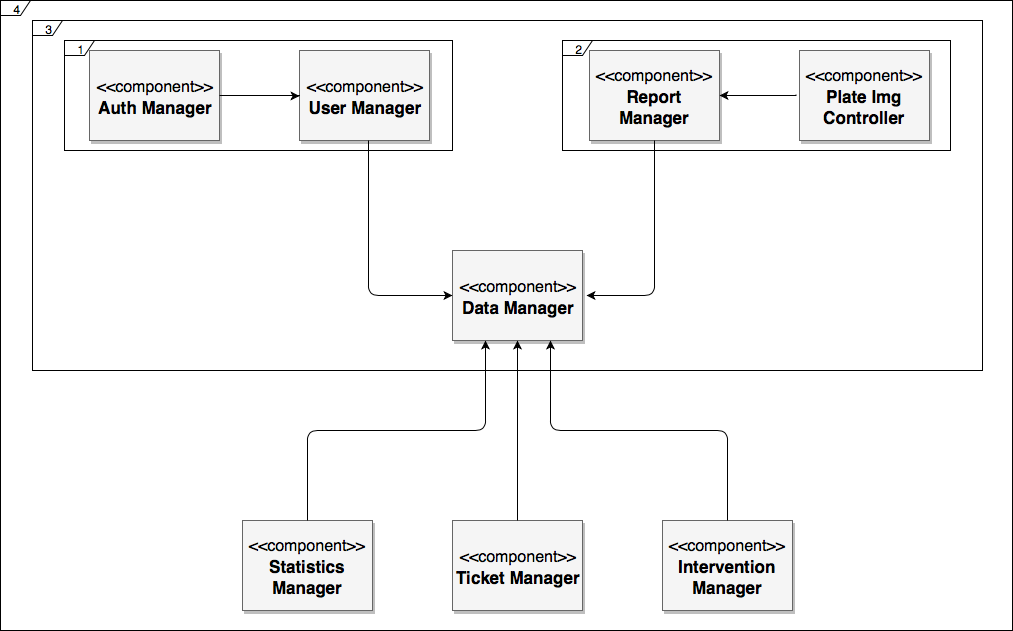
\includegraphics[scale=0.35]{Images/Diagrams/Testing/integration_diagram_1.png}
			\caption{Integration of the back-end components}
	\end{figure}
		\item Integration of the components of the front-end, the Presentation and the Data Manager, and test of the front-end operation;
		\begin{figure}[H]
			\centering
			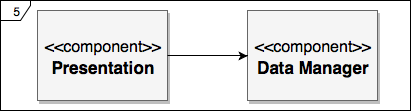
\includegraphics[scale=0.5]{Images/Diagrams/Testing/integration_diagram_2.png}
			\caption{Integration of the front-end components}
	\end{figure}
		\item Integration of back-end and front-end and test of the interactions between the two;
		\item Integration of components with external services interfaces and final test of the System.
	\end{enumerate}
	\begin{figure}[H]
			\centering
			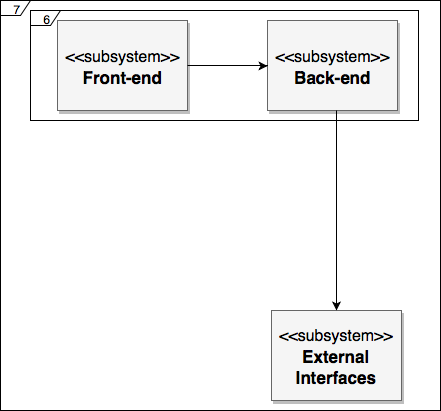
\includegraphics[scale=0.5]{Images/Diagrams/Testing/integration_diagram_3.png}
			\caption{Final integration}
	\end{figure}
	\pagebreak
		
% Effort - Section 6
\section{Effort Spent}
\begin{longtable}{| p{2 cm} | p{6 cm} | p{1 cm} |} 
			\hline
			{\bf Date} & {\bf Task} & {\bf Hours}\\
			\hline
			16/11/2019 & Pre-analysis & 1 \\
			\hline
			26/11/2019 & Meeting & 1 \\
			\hline
			30/11/2019 & Introduction & 1 \\
			\hline
			02/12/2019 & Overview & 2 \\
			\hline
			04/12/2019 & Component View & 3 \\
			\hline
			04/12/2019 & Meeting & 1 \\
			\hline
			05/12/2019 & Runtime View & 10 \\
			\hline
			06/12/2019 & Meeting & 1 \\
			\hline
			06/12/2019 & Component Interface & 3 \\
			\hline
			07/12/2019 & Requirements Traceability & 3 \\
			\hline
			07/12/2019 & Testing Plan & 2 \\
			\hline
			08/12/2019 & Architectural Styles & 2 \\
			\hline
			08/12/2019 & Revision & 2 \\
			\hline
			& & {\bf Total} \\
			\hline
			& & 32 \\
			\hline			
			\caption{Adriano Mundo's effort} 
\end{longtable}

\begin{longtable}{| p{2 cm} | p{6 cm} | p{1 cm} |} 
			\hline
			{\bf Date} & {\bf Task} & {\bf Hours}\\
			\hline
			16/11/2019 & Pre-analysis & 1 \\
			\hline
			26/11/2019 & Meeting & 1 \\
			\hline
			01/12/2019 & Overview & 1 \\
			\hline
			03/12/2019 & Component View & 1 \\
			\hline
			04/12/2019 & Meeting & 1 \\
			\hline
			05/12/2019 & Runtime View & 9 \\
			\hline
			06/12/2019 & Meeting & 1 \\
			\hline
			06/12/2019 & Component Interface & 2 \\
			\hline
			06/12/2019 & Architectural Styles & 1 \\
			\hline
			06/12/2019 & Requirements Traceability & 5 \\
			\hline
			08/12/2019 & Testing Plan & 4 \\
			\hline
			08/12/2019 & Revision & 2 \\
			\hline
			& & {\bf Total} \\
			\hline
			& & 29 \\
			\hline		
			\caption{Francesco Rota's effort} 

\end{longtable}
\pagebreak

\begin{longtable}{| p{2 cm} | p{6 cm} | p{1 cm} |} 
			\hline
			{\bf Date} & {\bf Task} & {\bf Hours}\\
			\hline
			16/11/2019 & Pre-analysis & 1 \\
			\hline
			26/11/2019 & Meeting & 1 \\
			\hline
			01/12/2019 & Overview & 3 \\
			\hline
			04/12/2019 & Meeting & 1 \\
			\hline
			04/12/2019 & Runtime View & 6 \\
			\hline
			06/12/2019 & User Interface Design & 5 \\
			\hline
			06/12/2019 & Meeting & 1 \\
			\hline
			07/12/2019 & Component Interface & 2 \\
			\hline
			07/12/2019 & Architectural Styles & 2 \\
			\hline
			08/12/2019 & Testing Plan & 2 \\
			\hline
			08/12/2019 & Revision & 2 \\
			\hline
			& & {\bf Total} \\
			\hline
			& & 26 \\
			\hline		
			\caption{Salvatore Fadda's effort} 
\end{longtable}
	
	
\end{document}
